\chapter[TRANSLATING: MATHEMATICAL EXPRESSIONS AND EQUATIONS]{TRANSLATING VERBAL PHRASES TO MATHEMATICAL
EXPRESSION \&\\ TRANSLATING OPEN SENTENCES TO
EQUATIONS}
\section*{INTRODUCTION}
This module presents a discussion on translating verbal phrases to mathematical expression
and translating open sentences to equation which includes assigning variable to one of the unknown
quantities, representing other unknowns in terms of same variable and forming mathematical
expression or equation from the given verbal phrase or open sentence. You will find in here several
examples and exercise to enhance your skill in translating verbal phrases to mathematical
expressions and vice versa. The skills and knowledge in translating verbal phrases to mathematical
phrase is very useful in solving application type problems.

\section*{OBJECTIVES}
After completing this module, you should be able to:
\begin{enumerate}
\item Explain the importance of translating verbal phrase to mathematical phrase in solving
application type problems;
\item Assign variable to one of the unknown quantities and represent the other unknown in terms
of same variable;
\item Translate verbal phrase to mathematical phrase;
\item Write word phrase for mathematical expression or equation; and
\item Apply it in solving application type problem.
\end{enumerate}
\section*{DISCUSSION}
In the course of your discussion with your family, you happen to ask your sibling about this riddle:
\textit{“Five years ago, I was half the age I will be in eight years. How old am I now?”}

It seems confusing on how to get it but in this lesson, we will apply some processes to solve such
kind of word problems. Let us first determine words and phrases that are commonly used to
represent an algebraic expression.
\begin{definition}[Algebraic expressions]
\Bold{Algebraic expressions} are made up of constants and variables connected by arithmetic operations. These operations include addition, subtraction, multiplication and division.
\end{definition}
Table \eqref{chap5tab:1} show examples of algebraic expressions.
\begin{figure}[!h]
\centering
\caption{Examples of algebraic expressions}
\begin{tabularu}{>{$}c<{$}>{$}c<{$}>{$}c<{$}}
\hline \hline
\text{Algebraic expression} & \text{Constant(s)} & \text{Variable(s)}\\
\hline
5x & 5 & x\\
3z-2 & 3\,\and 2 & z\\
\dfrac{2p+1}{5} & 2,1,\and 5 & p\\
5(3c+d) & 5, 4, \and 3 & c\and d\\
-5w-y & -5\and -1 & w\and y\\
\hline
\end{tabularu}
\label{chap5tab:2}
\end{figure}
In each of these algebraic expressions, we see that the constants and the variables are all attached
by arithmetic operations. So, we need to find out which phrases are used to stand for different
operations. Then, we can represent a verbal phrase as an algebraic expression.

It is important to remember that a variable is used to represent an unknown value. In some cases, a
phrase or sentence will tell us which variable we should use to represent the unknown value.
However, it is more common for the reader to create the variable using a let statement.
\begin{definition}[Let statement]
A \Bold{let statement} is used to help solve a word problem by creating a variable to represent the unknown value in the problem, e.g., ``Let $x=$ the unknown number.''
\end{definition}
Now that we know how to write a let statement, Let us apply this in the problem posed at beginning
of the lesson.
\begin{quote}
Let $a =$ Cousin Jesus' age now
\end{quote}
The following expressions all imply addition.

Let $n$ represent the unknown number.
\begin{center}
\begin{tabularu}{cc>{$}c<{$}}
\hline \hline
\text{Algebraic expression} & \text{Constant(s)} & \text{Variable(s)}\\
\hline
plus & 6 plus \textit{a number} & 6+n\\
added to & \textit{a number} added to 6 & 6+n\\
increased by & \textit{a number} increased by 6 & n+6\\
more than & 6 more than \textit{a number} & n+6\\
sum & the sum of 6 and \textit{a number} & 6+n\\
total & the total of 6 and \textit{a number} & 6+n\\
\hline
\end{tabularu}
\end{center}
The following expressions all imply subtraction.

Let $n$ represent the unknown number.
\begin{center}
\begin{tabularu}{ccc}
\hline \hline
Key Words & Word Expression & Algebraic Expression\\
\hline
\multirow{2}{*}{minus} & 5 minus \textit{a number} & $5-n$\\
 & \textit{a number} minus 5 & $n-5$\\
\hline
\multirow{2}{*}{diminished by} & \textit{a number} diminished by 5 & $n-5$\\
 & 5 diminished by \anumber & $5-n$\\
\hline
\multirow{2}{*}{decreased by} & \anumber{} decreased by 5 & $n-5$\\
 & 5 decreased by \anumber & $5-n$\\
\hline 
\multirow{2}{*}{subtracted from} & 5 subtracted from \anumber & $n-5$\\
 & \anumber{} subtracted from 5 & $5-n$\\
\hline
\multirow{2}{*}{less than} & 5 less than \anumber & $n-5$\\
 & \anumber{} less than 5 & $5-n$\\
\hline
\end{tabularu}
\end{center}
\begin{thinkback}
\textit{``Five minus a number"} and \textit{``a number minus five"} are not equivalent. There is no commutative property for subtraction since $5-7$ and $7-5$ are not equivalent. Remember that $5-7=-2$ and $7-5=+2$. Similarly, $5-n$ and $n-5$ are not equivalent. Expressions must be translated from English to algebraic form exactly.
\end{thinkback}
Try translating the following phrases on your own before looking at the answers.
\begin{example}
\Item Underline the key words in each expression, and then write the algebraic expression implied by each phrase below. Let $n=$ the number.

Word Expression\hfil Algebraic Expression

\begin{enumerate}
\item A number subtracted from 13
\item 16 more than a number
\item A number increased by 10
\item A number decreased by 10
\item The sum of a number and 5
\item 12 less than a number
\end{enumerate}
\tikz \node [rotate=180] {
\begin{inparaenum}[(a)]
\item $13-n$
\item $16+n$
\item $n+10$
\item $n-10$
\item $n+5$
\item $n-12$
\end{inparaenum}
};
\end{example}

Let's look at some expressions that imply multiplication.

This time, let $x$ represent the unknown number.

\begin{center}
\begin{tabularu}{cc>{$}c<{$}}
\hline \hline
Key Words & Word Expression & \text{Algebraic Expression}\\
\hline
times & 3 times a number & 3x\\
multiplied by & a number multiplied by 5 & 5x\\
product & the product of 3 and a number & 3x\\
twice & twice a number & 2x\\
double & double a number & 2x\\
triple & triple a number & 3x\\
of & 1/4 of a number & \frac{1}{4}x\\
\hline
\end{tabularu}
\end{center}
\begin{fact}
Multiplication is cummutative. Remember $3\cdot 4=4\cdot3$. However, when writing algebraic expressions, the constant is always written first. We write $4x$ rather than $x4$. Therefore a number multiplied by 4 is written $4x$ instead of $x4$.
\end{fact}
The last operation we need to look at is division.

The following expressions all imply division.

Let a represent the unknown number this time.
\begin{center}
\begin{tabularu}{cc>{$}c<{$}}
\hline \hline
Key Words & Word Expression & \text{Algebraic Expression}\\
\hline
\multirow{2}{*}{Quotient} & The quotient of 9 and a number & \frac{9}{n}\\
 & The quotient of a number and 9 & \frac{n}{9}\\
\multirow{2}{*}{Divided by} & A number divided by 9 & \frac{n}{9}\\
 & 9 divided by a number & \frac{9}{n}\\
\hline
\end{tabularu}
\end{center}
\begin{thinkback}
Division is not commutative. $\dfrac{2}{3}\neq\dfrac{3}{2}$. Likewise $\dfrac{7}{a}\neq\dfrac{a}{7}$.
\end{thinkback}
Notice that we no longer use the division symbol “$\div$”.

\yourown{}

\begin{center}
\begin{tabularu}{cc}
\hline \hline
Word Expression & \text{Algebraic Expression}\\
\hline
Three less than a number $r$ & \\
Four more than the number $x$ & \\
The quotient ten and a number $g$ & \\
Two-thirds of a number $a$ & \\
A number $c$ times 16 & \\
Nine less than a number $k$ & \\
\hline
\end{tabularu}

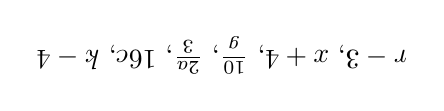
\begin{tikzpicture}
\node [rotate=180] {
$r-3$, $x+4$, $\frac{10}{g}$, $\frac{2a}{3}$, $16c$, $k-4$
};
\end{tikzpicture}
\end{center}

When we translate a word expression into an algebraic expression, it is very important to preserve
the order of operations.

The algebraic expression, $3(x + 2)$, is not equivalent to the algebraic expression, $3x + 2$.

The algebraic expressions on the right represent the word expressions on the left.
The variable n will be used to hold the place of the unknown number.

\begin{center}
\begin{tabularu}{c>{$}c<{$}}
\hline
Word Expression & \text{Algebraic Expression}\\
\hline
four times a number & 4x\\
five times the sum of a number and eight & 5(x + 8) \\
Ana's age in 12 years if her present age is $a$ & a + 12\\
5.2 times the square of the length of the radius & 5.2r^2\\
The sum of two consecutive integers if $r$ is the first integer & r + (r + 1)\\
Thrice the difference of a number and one & 3 (x - 1)\\
Fe's age 9 years ago & f-9\\
A given height subtracted from nine times that height & 9h-h\\
\hline
\end{tabularu}
\end{center}

\yourown{}

\begin{center}
\begin{tabularu}{cc}
\hline \hline
Word Expression & Algebraic Expression\\
\hline
\parbox[t][]{0.5\linewidth}{
\begin{enumerate}
\item The difference of 7 and twice a number $y$
\item Twice the difference of 7 and a number $y$
\item Twice the difference of a number $y$ and 7
\item Rey's age in $h$ years if he is 11 now
\end{enumerate}
}
 & \\
\hline
\end{tabularu}
\end{center}
We are already done with translating phrases into algebraic expressions, next is to complete the
mathematical sentence in order to create an algebraic equation.
\begin{definition}[Algebraic equation]
An \Bold{algebraic equation} has an algebraic expression set equal to a number or another expression, e.g., $3x+2=7$, $3n-7=4n$, and $\dfrac{a}{5}+5=10a-8$.
\end{definition}
The key word for translating complete sentences into an equation is the word “is”. All forms of the
word “is” represent the equal sign in an equation.

In this example, let us express the mathematical sentence into an algebraic equation.
“Five years ago, I was half the age I will be in eight years.”
\begin{quote}
\begin{tabular}{l>{$}l<{$}}
Five years ago & a-5\\
I was half the age & \frac{1}{2}\\
I will be in eight years & a+8\\
\end{tabular}
\end{quote}
So, now we will write this sentence as an algebraic equation.
\begin{equation*}
a-5=\frac{1}{2}(a+8)
\end{equation*}
Let's try one more together.
\begin{example}
\Item Five more than twice a number is three times the difference of that number and two.

\textbf{Solution}: 

Let $n=$ the number.

Five \Underline{more than twice} a number \Underline{is} three \Underline{times} the \Underline{difference} of that number and two.

The mathematical equation is $2n + 5 = 3 (n-2)$.
\end{example}
\yourown{}
\begin{center}
\begin{tabular}{p{0.4\linewidth}c}
\hline \hline
\multicolumn{1}{c}{Sentence} & Equation \\
Thrice the sum of eight and a number is twelve less than that same number
 & \\
Nine years from now, Ana will be four times her age from 5 years ago. & \\
\end{tabular}
\end{center}
\begin{example}
\Item Three consecutive integers sum to 99.

\Solution

Consecutive integers increase by one each time.

Let
\begin{tabular}[t]{@{}>{$}r<{\,$}@{}l}
x = & the first integer\\
x + 1 = & the second integer\\
x + 2 = & the third integer\\
\end{tabular}

We add our three integers and set that equal to 99.
\begin{equation*}
x + (x + 1) + (x + 2) = 99
\end{equation*}
\end{example}
Let’s try one that is a little harder.
\begin{example}
\Item Jessica has Php 3.15 in 25-centavo, 10-centavo, and 5-centavo coins. She has twice as many 5-
centavo coins as 10-centavo coins as and two less 25-centavo than 5-centavo.

\Solution

Let
\begin{tabular}[t]{@{}>{$}r<{\,$}@{}l}
d = & number of 10-centavo\\
2d = & number of 5-centavo\\
2d - 2 = & number of 25-centavo\\
\end{tabular}
\end{example}

\yourown{Translate the following sentences to equations.}
\begin{center}
\begin{tabularu}{p{0.4\linewidth}c}
\hline \hline
\multicolumn{1}{c}{Sentence} & Equation\\
\hline
Three consecutive integers sum to 96. & \\
Ana has Php 2.00 in the denomination of 25-centavo, 10-centavo, and 5-
centavo coins. The number 10-centavo is twice the number of 5-centavo and
the number of 25-centavo is thrice the number of 5-centavo coins. Form an
e2quatiuon representing the total amount of her coins. & \\
\hline
\end{tabularu}
\end{center}
Here is a summary table which lists some key words and phrases that are used to describe common
mathematical operations.
\begin{longtable}{p{0.2\linewidth}p{0.2\linewidth}p{0.3\linewidth}>{$}p{0.125\linewidth}<{$}}
\kill
\caption{Common key words and phrases for mathematical operations}\label{chap5tab:1}\\
\hline \hline
%\endfooter
Operation & Key Word/Phrase & Example & Translation \\
\hline \hline
\endfirsthead
\caption[]{(continued)}\\
\hline \hline
Operation & Key Word/Phrase & Example & Translation \\
\hline \hline
\endhead
\hline
\multicolumn{4}{r}{{Continued on next page}} \\
\endfoot
\hline
\endlastfoot
Addition ($+$) & plus & a number plus two & n+2\\
 & more than & Six more than a number & n+6\\
 & the sum of & The sum of a number and three & n+3\\
 & the total of & the total of five and a number & n+5\\
 & increased by & A number increased buy one & n+1\\
 & added to & Thirteen added to a number & n+13\\
\hline \hline
Subtraction ($-$) & minus & A number minus eight & n-8\\
 & less than & Two less than a number & n-2\\
 & the difference of & The difference of a number and five & n-5\\
 & less & Eleven less number & 11-n\\
 & decreased by & A number decreased by six & n-6\\
 & subtracted by & Three subtracted by a number & 3-n\\
\hline \hline
Multiplication ($\times$) & times & Three times a number & 3n\\
 & the product of & The product of five and a number & 5n\\
 & twice, double  & Twice a number, double a number  & 2n\\
 & multiplied by  & A number multiplied by four 			& 4n\\
 & of						  & Two-fifths of a number 					& \frac{2n}{5}\\
\hline \hline
Division ($\div$) & The quotient of & The quotient of 2 and a number & \frac{2}{n}\\
 & Divided by & Thirty divided by a number & \frac{30}{n}\\
 & The ratio of & The ratio of a number and six & \frac{n}{6}\\
\hline \hline 
Powers ($x^n$) & the square of & The square of a number or number squared & n^2\\
 & the cube of & The cube of a number or number cubed & n^3\\
\hline \hline
Equals ($=$) & equals & Three less than a number equals nine & n-3=9\\
 & is & Two times a number is 14 & 2n=14\\
 & is the same as & Fifteen is the same as thrice a number & 15=3n\\
 & yields & A number added to one yields four & n+1=4\\
 & amounts to & Six less than a number amounts to twenty-four & n-6=24\\
\hline 
\end{longtable}


\section*{SUGGESTED ACTIVITIES}
\subsection*{Activity 1: Translate each word phrase to algebraic expression}
\begin{enumerate}
\item The sum of $n$ and 5. 
\item The product of $x$ and $y$ 
\item Nine more than a number 
\item Twice of a number 
\item Three-fourths of a number 
\item A number decreased by 8 
\item 10 more than the unknown 
\item The quotient of a number and 3 
\item Six more than thrice a number 
\item Five times the sum of a number and 4 
\item The ratio of $x$ and $2y$
\item One less than 9 times a number 
\item Five times a number increased by 4 
\item One more than a number 
\item The product of twice a number and 8 increased by six 
\end{enumerate}
\Answers
\begin{enumerate}
\item $n+5$
\item $xy$
\item $x+9$
\item $2x$
\item $\frac{3x}{4}$
\item $x-8$
\item $x + 10$
\item $\frac{x}{3}$
\item $3x + 6$
\item $5(x +4)$
\item $\frac{x}{2y}$
\item $9x-1$
\item $5x + 4$
\item $x+1$
\item $(2x)(8) + 6$
\end{enumerate}
\subsection*{Activity 2: Translating Exercise}
Write a word phrase for each algebraic expression: (Note: There are many ways in writing a word
phrase for certain algebraic expression)
\begin{enumerate}
\item $\frac{2}{y}$
\item $x + 4$
\item $x-6$
\item $7x + 4$
\item $2x-6$
\item $3(n + 2)$
\item $52-4a$
\item $x^2+2$
\item $\frac{2x+3}{7}$
\item $5-\frac{3}{x}$
\end{enumerate}
\Answers
\begin{enumerate}
\item The quotient of 2 and $y$.
\item A number increased by 4.
\item Six less than a number.
\item Four more than seven times a number.
\item Twice a number less than six.
\item Thrice the sum of n and 2.
\item Fifty-two decreased by four times a number
\item The square of $x$ added to 2.
\item The quotient of twice of $x$ added to 3 and 7.
\item Five decreased by the quotient of 3 and $x$.
\end{enumerate}
\subsection*{Activity 3: Translating Activity 3}
\begin{enumerate}
\item $7x +3 = 17$
\item $4(x + 5) < 20$
\item $(3x)(8) - 7 =31$
\item $x+\frac{x}{3}\ge 16$
\item $8 - 4x = 7$
\item $x + (x + 2) = 14$
\item $\frac{x}{5}-100$
\item $3(x + 9) = 36$
\item $3x + 9 = 36$
\item $2x + 3x = 75$
\end{enumerate}
\Answers
\begin{enumerate}
\item Seven times a number increased by 3 is 17.
\item Four times the sum of a number and five is less than twenty.
\item The product of thrice a number and 8 decreased by 7 is 31.
\item A number increased one-third of itself is greater than or equal to 16.
\item The difference of eight and four time a number is 7.
\item The sum of two consecutive even integers is 14.
\item The quotient of a number and 5 decreased by 15 is 100.
\item Thrice the sum of a number and 9 is 36
\item The sum of thrice a number and 9 is 36.
\item Twice a number added by thrice of same number is 75.
\end{enumerate}
\subsection*{Activity 4: Translating Activity 4}
Give the equation/inequality for the given sentence/situation.
\begin{enumerate}[A.]
\item Number Problems
	\begin{enumerate}
	\item Twice a number increased by 12 is 48.
	\item The difference of twice a number and 5 is 7.
	\item The product of a number and 11 is less than or equal to 165.
	\item Decreasing a number by 25 gives 42.
	\item The larger number is four more than the smaller number. If their sum is 72, form an equation stating their sum.
	\item The sum of two numbers is 92. One number is twelve less than the other. Find numbers. 
	\item The sum of two consecutive integers is sixty-three.
	\item A number added to half of itself is 9. 
	\end{enumerate}
\item Age Problems 
	\begin{enumerate}
	\item Rona's age five years ago was 25. 
	\item Ten less thrice of Fe's age is 58. 
	\item Cora is three years older than Din. If the sum of 
    their ages is 35 years, form an equation representing 
    the sum of their ages. 
	\item Ana is five years older than Jen. If the sum of their 
    ages is 11, form an equation stating the sum of their 
    ages.
	\end{enumerate}
\item Money Problems
	\begin{enumerate}
	\item Fe saves 5-centavo and 10-centavo coins. If she has 28 coins worth Php 2.60, form an equation
representing the total amount of her coins.
	\item Jen has 26 coins in the denomination of 5 centavos and 25 centavo. If the total amount of her coins is Php 3.10, form an equation representing the total amount of her coins.
	\end{enumerate}
\item Investment Problem
	\begin{enumerate}
	\item An amount of Php 10,000 is invested at 3.5\% simple interest for one year. Form an equation representing the interest.
	\item Len invested some money at 3\% and Php 4000 less than that amount at 5\%. The two investments produced a total of Php 200 interest in one year. Form an equation representing the total interest of the two investments.
	\end{enumerate}
\item Mixture Problem
	\begin{enumerate}
	\item A mechanic added 25\mL of water to 125\mL of a 20\% solution of antifreeze in water. Form an equation representing the concentration of antifreeze in the new solution?
	\item A certain amount of water was added to a 50\mL solution of 25\% acid in water. If the resulting mixture has concentration of 10\% acid, form an
equation representing the concentration of the new
mixture.
	\end{enumerate}
\item Uniform Motion Problem
	\begin{enumerate}
	\item Two trains leave from a station at the same time. They travel in opposite directions, one at 62 km/h and the other at 48 km/h. If they are 550 km after certain time, form an equation representing the total distance covered by the two trains.
	\item Two hikers leave on same the place at the same time and travels in opposite direction, one travels 2 kph faster than the other. If they 168 km apart after 4 hours, form an equation representing the total distance covered by the hikers after 4 hours.
	\end{enumerate}
\end{enumerate}
\subsection*{Activity 5: Math BINGO}\label{chap5sec:1}
\subsubsection*{Level 1}
\begin{enumerate}[Step 1.]
\item The participants will have to translate the verbal phrases to mathematical expressions and
randomly place them on their bingo cards.
\item The facilitators will check if everybody has finished accomplishing their bingo cards.
\item The resource person will announce the pattern to be accomplished. There could be more
than 1 winning pattern for higher chances of winning.
\item The resource person will randomly read verbal phrase one at a time and the participants will
mark the corresponding mathematical expression on their bingo card.
\item If a pattern is completed, the participant will just have to “announce”. The facilitator and
resource person will verify the correctness of the bingo card. If there is a wrong entry, the
participant is disqualified and the activity continues. Otherwise, the winner is proclaimed.
\item The game may continue for the other patterns or the game may be restarted for a different
pattern.
\end{enumerate}
\begin{figure}[!h]
\centering
\caption{Bingo Cards for Activity \eqref{chap5sec:1}}
\begin{tabular}{|c|c|c|c|c|c|c|}
\hline
\multicolumn{7}{|c|}{Game 1}\\
\hline
\multicolumn{7}{|c|}{}\\
\cline{2-6}
\hphantom{.} & P & I & S & A & Y & \hphantom{.}\\
\cline{2-6}
 & & &\cellcolor{\bingo} & & & \\ \cline{2-6}
 & & &\cellcolor{\bingo} & & & \\ \cline{2-6}
 & & &\cellcolor{\bingo} & & & \\ \cline{2-6}
 & & &\cellcolor{\bingo} & & & \\ \cline{2-6}
 & & &\cellcolor{\bingo} & & & \\ \cline{2-6}
\multicolumn{7}{|c|}{}\\
\hline
\end{tabular}
\hfil 
\begin{tabular}{|c|c|c|c|c|c|c|}
\hline
\multicolumn{7}{|c|}{Game 1}\\
\hline
\multicolumn{7}{|c|}{}\\
\cline{2-6}
\hphantom{.} & P & I & S & A & Y & \hphantom{.}\\
\cline{2-6}
 &\cellcolor{\bingo} & & & & \cellcolor{\bingo} & \\ \cline{2-6}
 & & & & & & \\ \cline{2-6}
 & & &\cellcolor{\bingo} & & & \\ \cline{2-6}
 & & & & & & \\ \cline{2-6}
 & \cellcolor{\bingo} & & & & \cellcolor{\bingo} & \\ \cline{2-6}
\multicolumn{7}{|c|}{}\\
\hline
\end{tabular}
\hfil 
\begin{tabular}{|c|c|c|c|c|c|c|}
\hline
\multicolumn{7}{|c|}{Game 1}\\
\hline
\multicolumn{7}{|c|}{}\\
\cline{2-6}
\hphantom{.} & P & I & S & A & Y & \hphantom{.}\\
\cline{2-6}
 &\cellcolor{\bingo} & & & & \cellcolor{\bingo} & \\ \cline{2-6}
 & & \cellcolor{\bingo} & & \cellcolor{\bingo} & & \\ \cline{2-6}
 & & &\cellcolor{\bingo} & & & \\ \cline{2-6}
 & & \cellcolor{\bingo} & & \cellcolor{\bingo} & & \\ \cline{2-6}
 & \cellcolor{\bingo} & & & & \cellcolor{\bingo} & \\ \cline{2-6}
\multicolumn{7}{|c|}{}\\
\hline
\end{tabular}
\label{chap5fig:1}
\end{figure}

\begin{center}
\begin{longtable}{p{0.5\linewidth}>{\centering\arraybackslash$}p{0.3\linewidth}<{$}}
\kill
\caption{Questions for \eqref{chap5fig:1}}\label{chap5tab:3}\\
\hline \hline
\parbox[t]{\linewidth}{\centering
Verbal Phrases\\
(In the Bingo Box)
} & 
\parbox[t]{\linewidth}{\centering
Mathematical Expressions\\
(Card Entries)
}\\
\hline \hline
\endfirsthead
\caption[]{(continued)}\\
\hline \hline
\parbox[t]{\linewidth}{\centering
Verbal Phrases\\
(In the Bingo Box)
} & 
\parbox[t]{\linewidth}{\centering
Mathematical Expressions\\
(Card Entries)
}\\
\hline \hline
\endhead

\hline \hline
\multicolumn{2}{r}{{Continued on next page}} \\
\endfoot

\hline \hline
\endlastfoot
a number decreased by seventy-eight & n-78\\
the difference between a number and twenty-seven & n-27\\
the quotient of a number and fifty-three & \frac{n}{53}\\
the sum of four and a number & 4+n\\
the quotient of sixty-five and a number & \frac{65}{n}\\
a number increased by fifty-eight & n+58\\
the difference between thirty-six and a number & 36-n\\
a number added to fifty-six & 56+n\\
seventy-three less than a number & n-73\\
the product of a number and forty-four & 44n\\
a number decreased by thirty-three & n-33\\
twenty-eight times a number & 28n\\
the sum of twenty-three and a number & 23+n\\
the quotient of a number and seventy-nine & \frac{n}{79}\\
the difference between a number and fifty-nine & n-59\\
the sum of a number and thirty-seven & n+37\\
the quotient of sixty-one and a number & \frac{61}{x}\\
a number increased by ninety-three & x+93\\
the product of thirty-two and a number & 32x\\
the product of twenty-five and a number & 25x\\
the difference between a number and eight & x-8\\
nine more than a number & x+9\\
fifty-nine times a number & 59x\\
the quotient of a number and ninety-seven & \frac{x}{97}\\
seventeen times a number & 17x\\
the sum of sixty-one and a number & 61+x\\
a number decreased by eighty-six & x-86\\
the difference between ninety and a number & 90-x\\
eighty-one less than a number & x-81\\
The sum of a number and 3 & x+3\\
The product of a number and 3 & 3x\\
The sum of two numbers & x+y\\
Three times the sum of two numbers & 3(x+y)\\
Three times a number & 3x\\
Three less than a number & x-3\\
A number, less 3 & x-3\\
Three more than a number & x+3\\
A number, plus 3 & x+3\\
The square of a number & x^2\\
The square of three times a number & (3x)^2\\
Three times the square of a number & 3x^2\\
One-third of a number & \frac{x}{3}\\
One less than 3 times a number & 3x-1\\
Two more than 5 times a number & 5x+2\\
The square of the sum of two numbers & (x+y)^2\\
The sum of the squares of two numbers & x^2+y^2\\
\hline
\end{longtable}
\end{center}

\subsection*{Activity 6: Bingo Activity 2}\label{chap5sec:2}
\begin{figure}[!ht]
\centering
\caption{Bingo Cards for Activity 2}
\begin{tabular}{|c|c|c|c|c|c|}
\hline
\multicolumn{6}{|c|}{|Game 4|}\\
\cline{2-5}
 & M & A & T & H & \\ \cline{2-5}
 & & & & & \\ \cline{2-5}
 & & \cellcolor{\bingo} & \cellcolor{\bingo} & & \\ \cline{2-5}
 & & \cellcolor{\bingo} & \cellcolor{\bingo} & & \\ \cline{2-5}
 & & & & & \\ \cline{2-5}
\multicolumn{6}{|c|}{}\\
\hline
\end{tabular}
\hfil 
\begin{tabular}{|c|c|c|c|c|c|}
\hline
\multicolumn{6}{|c|}{|Game 5|}\\
\cline{2-5}
 & M & A & T & H & \\ \cline{2-5}
 & &\cellcolor{\bingo} & \cellcolor{\bingo} & & \\ \cline{2-5}
 &\cellcolor{\bingo} & & & \cellcolor{\bingo} & \\ \cline{2-5}
 & \cellcolor{\bingo} & & & \cellcolor{\bingo} & \\ \cline{2-5}
 & & \cellcolor{\bingo} & \cellcolor{\bingo} & & \\ \cline{2-5}
\multicolumn{6}{|c|}{}\\
\hline
\end{tabular}
\label{chap5fig:2}
\end{figure}
Follow the same procedures in Activity \eqref{chap5sec:1}.

\begin{center}
\begin{longtable}{p{0.5\linewidth}>{\centering\arraybackslash$}p{0.3\linewidth}<{$}}
\kill
\caption{Questions for \eqref{chap5fig:2}}\label{chap5tab:4}\\
\hline \hline
\parbox[t]{\linewidth}{\centering
Verbal Phrases\\
(In the Bingo Box)
} & 
\parbox[t]{\linewidth}{\centering
Mathematical Expressions\\
(Card Entries)
}\\
\hline \hline
\endfirsthead
\caption[]{(continued)}\\
\hline \hline
\parbox[t]{\linewidth}{\centering
Verbal Phrases\\
(In the Bingo Box)
} & 
\parbox[t]{\linewidth}{\centering
Mathematical Expressions\\
(Card Entries)
}\\
\hline \hline
\endhead

\hline \hline
\multicolumn{2}{r}{{Continued on next page}} \\
\endfoot

\hline \hline
\endlastfoot
A number increased by nine is fifteen. & \\
Twice a number is eighteen. & \\ \hline
Four less than a number is twenty. & \\ \hline
A number divided by six is eight. & \\ \hline
Twice a number, decreased by twenty-nine, is seven. & \\ \hline
Thirty-two is twice a number increased by eight. & \\ \hline
The quotient of fifty and five more than a number is ten. & \\ \hline
Twelve is sixteen less than four times a number. & \\ \hline
Eleni is x years old. In thirteen years she will be twenty-four years old. & \\ \hline
Each piece of candy costs 25 cents. The price of h pieces of candy is & \\ \hline
Suzanne made a withdrawal of d dollars from her savings account. Her old balance was \$350, and her new balance
is & \\ \hline
A large pizza pie with 15 slices is shared among p students so that each student's share is 3 slices. & \\ \hline
Lorene has some nickels, twice as many dimes as nickels, and half as many quarters as nickels. All total she has 77 coins. & \\ \hline
Jack is 25 years younger than his mother. Together, their ages add up to 89. & \\ \hline
Cucumbers cost 15\textcent{} each and tomatoes costs 9\textcent{} each. Mom buys six more tomatoes than cucumbers. Her total bill is \$1.26. & \\ \hline
Marie bought 12 fruits, of which there were x apples, five fewer oranges than apples, and one pineapple. & \\ \hline
Tara is twice as old as Gwen. Their sister, Amy, is 5 years older than Gwen. If the sum of their ages is 29 years, find each of their ages. & \\ \hline
Carol is 25 years older than her cousin Amanda. Cousin Bill is 3 times as old as Amanda. The sum of their ages is 90. Find each of their ages. & \\ \hline
Derrick is 5 less than twice as old as Brandon. The sum of their ages is 43. How old are Derrick and Brandon? & \\ \hline
Beth’s mom is 6 times older than Beth. Beth’s dad is 7 years older than Beth’s mom. The sum of their ages is 72. How
old are each of them? & \\ \hline
Ruby is 2 years more than three times as old as her son, Raul. If the difference between their ages is 26, how old are Ruby and Raul? & \\ \hline
Sam is ten less than 3 times as old as Alex. If the difference between their ages is 28, how old is Sam and Alex. & \\ \hline
Eileen is 6 years older than Karen. John is three times as old as Karen. The sum of their ages is 56. How old are Eileen, Karen and John? & \\ \hline
Taylor is 18 years younger than Jim. Andrew is twice as old as Taylor. The sum of their ages is 26. How old are Taylor, Jim and Andrew? & \\ \hline
Jick is 3 years less than four times as old as Jall. If the difference between their ages is 72, how old are Jick and Jall? & \\ \hline
Rufio is 15 years younger than Rafe. Rafe is four times older than Raquel. If the sum of their ages is 48 then how old are they? & \\ \hline
Robert and Roberta are twins. The product of their ages is 196. & \\ \hline
\hline
\end{longtable}
\end{center}